% This is samplepaper.tex, a sample chapter demonstrating the
% LLNCS macro package for Springer Computer Science proceedings;
% Version 2.20 of 2017/10/04
%
\documentclass[runningheads]{llncs}
%
\usepackage{graphicx}

%custom packages
\usepackage{amsmath}
\usepackage{amssymb}
\usepackage{cite}
\usepackage{subfig}
\usepackage{breqn}
\usepackage[labelfont=bf,labelsep=period]{caption}

\usepackage[utf8]{inputenc}
\inputencoding{utf8}
\usepackage[english]{babel}

\DeclareMathOperator*{\argmax}{arg\,max}
\DeclareMathOperator*{\argmin}{arg\,min}
\DeclareMathOperator{\sign}{sign}
% Used for displaying a sample figure. If possible, figure files should
% be included in EPS format.
%
% If you use the hyperref package, please uncomment the following line
% to display URLs in blue roman font according to Springer's eBook style:
% \renewcommand\UrlFont{\color{blue}\rmfamily}

\begin{document}
%
\title{Parallel global optimization algorithm with uniform convergence
for solving a set of constrained global optimization problems\thanks{This study was supported
by the Russian Science Foundation, project No.\,16-11-10150.}}
%
\titlerunning{Parallel global optimization algorithm with uniform convergence}
% If the paper title is too long for the running head, you can set
% an abbreviated paper title here
%
\author{Vladislav Sovrasov\and
Konstantin Barkalov
}
%
\authorrunning{V. Sovrasov et al.}
% First names are abbreviated in the running head.
% If there are more than two authors, 'et al.' is used.
%
\institute{Lobachevsky State University of Nizhni Novgorod, Nizhni Novgorod, Russia
\email{sovrasov.vladislav@itmm.unn.ru},
\email{konstantin.barkalov@itmm.unn.ru}
}
%
\maketitle              % typeset the header of the contribution
%
\begin{abstract}
In the present work, an extension of global optimization algorithm for solving a set of problems
simultaneously onto a case of problems with non-convex constraints is considered. The property
of uniform convergence inherent to the algorithm allows distributing the computation resources
in the optimal way since the errors of numerical solutions decrease with approximately equal
rates in all problems in the course of the execution of the algorithm. The algorithm assigns a
priority to each problem and performs the computations of the objective functions in several
problems in parallel at every iteration. Upon stop of the method at arbitrary time moment,
solutions of similar quality would be obtained in all problems of the series being solved. A series
of several problems arises if the global optimization problem has a discrete parameter or, for
example, in solving a multicriteria optimization problem using criteria convolution. The
considered algorithm employs Peano-type space-filling curves for the reduction of the
multidimensional optimization problems to the one-dimensional ones.  The efficiency of the
implemented algorithm was tested using the sets of artificially generated global optimization
problems as well as in solving a series of problems obtained as a result of scalarization of a
multicriteria optimization  problem. Also, the numerical experiments confirmed the uniform
convergence of the proposed method.

\keywords{Global optimization \and Non-convex constraints \and Uniform convergence \and Derivative-free optimization
\and Parallel computing.}
\end{abstract}
%
%
%

\section{Introduction}
\label{sec-intro}
Global optimization problems with non-convex constraints are considered traditionally to be one
of the most difficult optimization problems.
 The finding of the global minimum of a function of several variables appears to be more
difficult often than a local optimization in a thousand-dimensional space.
For the latter, application of the simplest gradient descent method may appear to be enough,
whereas to \textit{guarantee} the finding of the global optimum the optimization
methods have to accumulate the information on the behaviour of the objective function in the
whole search domain \cite{Jones2009,Paulavicius2011,Evtushenko2013,Strongin2000}.
The solving of a series of such problems at limited computational resources is even more
difficult problem: besides the search of the global extremum, it is necessary to distribute the
computational resources in such a way that the location of the global extremum would be
estimated with approximately equal quality in all problems being solved at once.
Usually, a series of \(q\) problems is solved either sequentially or in parallel by portions of \(p\ll
q\) problems where \(p\) is a number of parallel computational devices.
Such an approach leads to a situation when at every time moment until the stop of computations
some problems remain, in which the estimate of the global optimum is not obtained yet whereas
in the problems from the beginning of the list the optimum may be estimated even with excess
precision.

In the present work, a generalization of parallel global optimization method for simultaneous
solving of a set of problems developed earlier in Lobachevsky State University of Nizhni Novgorod
\cite{BarkalovStrongin2018} onto the case of non-convex constraints is considered. To account
for the constraints, the index scheme \cite{Strongin2000,Pugliese} is applied allowing working with
partially defined objective function and constraints and featured by efficiency comparable to other
approaches \cite{BarkalovLebedev2017}. The convergence of the algorithm to the global
optimizers in all problems was proved theoretically, the efficiency of the implemented
algorithm was demonstrated by solving sets of problems generated by a special mechanism
generating the sets of problems of predefined dimensionality with predefined number of
non-convex constraints \cite{GergelBarkalov2019}.
Besides the problems generated artificially, the considered method was tested also on a set of
problems arising when solving a multicriteria optimization problem with nonlinear constraints by
criteria convolution method \cite{Ehrgott2005}.

The paper is structured as follows. In Section \ref{sec:problem}, the statement of the problem to
be solved is considered. Then, in Section \ref{sec:method}, a description of the parallel
optimization method is given. The sufficient conditions of convergence of the considered
method are given in Section \ref{sec:conv_method}.
The results of the numerical experiments confirming the efficiency of considered method are
presented in Section \ref{sec:exps}.
In Conclusion, a short summary of the results obtained in the present study is given and the
directions of further effort on the improvement of the software implementation of the
considered method are outlined.


\section{Global optimization problem statement}
\label{sec:problem}
In this work we consider the following
problem: to find the global minimum of an \(N\)-dimensional function \(\varphi(y)\) in
a hyperinterval $D$
\begin{equation}
\label{eq:task}
\varphi(y^*)=\min\{\varphi(y):y\in D\},
\end{equation}
\begin{displaymath}
D=\{y\in \mathbf{R}^N:a_i\leqslant x_i\leqslant{b_i}, 1\leqslant{i}\leqslant{N}\}.
\end{displaymath}
In order to construct an estimate of the global minimum based on a finite number of
computations of the function values, the rate of variation of \(\varphi(y)\) in \(D\) is required to
be limited.
As a rule, the Lipschitz condition
\begin{displaymath}
\label{lip}
|\varphi(y_1)-\varphi(y_2)|\leqslant L\Vert y_1-y_2\Vert,y_1,y_2\in D,0<L<\infty,
\end{displaymath}
is accepted as such a limitation.

There are various methods solving the considered multidimensional problem directly
\cite{SergeyevKvasov2017, Jones2009} as well as efficient methods for solving the univariate problems \cite{Norkin1992, Strongin2000}.
In the present work, a one-dimensional method is considered, which is applied together with the
dimensionality reduction scheme.
The use of space-filling curve (or \textit{evolvent}) $y(x)$, where
\begin{equation}
\label{cube}
\lbrace y\in \mathbf{R}^N:-2^{-1}\leqslant y_i\leqslant 2^{-1},1\leqslant i\leqslant
N\rbrace=\{y(x):0\leqslant x\leqslant 1\},
\end{equation}
 is a classical scheme of reduction of the
dimensionality of the initial problem for the global optimization algorithms
\cite{Sergeyev2013}.
A mapping of the type (\ref{cube}) allows reducing a multidimensional problem to a univariate one at the expense of worsening its properties. In particular, the
one-dimensional function \(\varphi(y(x))\) is not lipschitzian but h\"{o}lderian one:
\begin{displaymath}
\label{holder}
|\varphi(y(x_1))-\varphi(y(x_2))|\leqslant H{|x_1-x_2|}^{\frac{1}{N}}, \; x_1,x_2\in[0,1],
\end{displaymath}
where the H\"{o}lder constant \(H\) is related to the Lipschitz one \(L\) by the relation
\begin{displaymath}
  H=2L\sqrt{N+3}.
\end{displaymath}

The feasible domain can also be defined by the constraints that essentially complicate the problem.
The problem statement in this case will take the following form:
\begin{equation}
  \label{eq:constrained_problem}
  \varphi(y^*)=\min\{\varphi(y):y\in D \cap \{y: g_j(y)\leqslant 0, 1\leqslant j\leqslant m\}\}.
\end{equation}

Let us denote \(g_{m+1}(y)=\varphi(y)\). Hereafter, we will assume all functions
\(g_k(y),1\leqslant k \leqslant m+1\),
to satisfy the Lipschitz condition in some hyperinterval including \(D\).

Further, let us consider solving a series of \(q\) problems of the kind
(\ref{eq:constrained_problem}):
\begin{equation}
  \label{eq:many_problems}
  \min\left\{\varphi_1(y), y\in D_1 \right\}, \min\left\{\varphi_2(y), y\in D_2\right\},...,
\min\left\{\varphi_q(y), y\in D_q\right\}.
\end{equation}

\section{Description of the global optimization method}
\label{sec:method}

Taking into account the dimensionality reduction scheme (\ref{cube}), let us assume when
describing the method that it is required to find the global minimum of the function \(\varphi(x),
x\in[0,1]\), satisfying the H\"{o}lder condition with the constraints \(g_j(x)\) also satisfying this
condition in the interval \([0,1]\).

The index algorithm of global search (IAGS) for solving the one-dimensional problems
%(\ref{eq:constrained_problem})
considered here implies the constructing of a sequence of points
\(x_k\), which the values of the minimized function or of the constraints \(z_k = g_s(x_k)\) are
computed in.
To account for the latter, the index scheme \cite{Strongin2000} was used.
Let \(Q_0=[0,1]\). The constraint having the index \(j\) is satisfied in all points of the domain
\begin{displaymath}
  Q_j=\left\{x\in [0,1]:g_j(x)\leq 0\right\},
\end{displaymath}
which is called feasible for this constraint.
At that, the feasible domain \(D\) of the initial problem is defined by the equality
 \(D=\cap _{j=0}^{m}Q_{j}\).
A trial in the point \(x\in [0,1]\) consists in a sequence computing of the values
\(g_{1}(x),...,g_{\nu }(x)\)
where the values of the indices \(\nu\) are defined by the conditions:
\(x\in Q_{j},0\leqslant j<\nu ,x\notin Q_{\nu }\).
The finding of the first violation of any constraint terminates the trial at the point \(x\).
In the case when the point \(x\) is feasible, i.e. \(x\in D\), the trial includes the computing of all
functions of the problem.
At that, the value of the index is accepted to be equal to the magnitude \(\nu =m+1\).
The pair \(\nu =\nu (x), z=g_{\nu }(x)\) where the index \(\nu\) falls into the borders \(1\leqslant
\nu \leqslant m+1\) is called the result of the trial at the point \(x\).

Such an approach to conducting the trials allows reducing the initial problem with functional
constraints to an unconstrained problem of minimization of a discontinuous function:

\begin{displaymath}
  \begin{array}{lr}
    \psi (x^{*})=\min_{x\in [0,1]}\psi (x), \\
    \psi (x)={\begin{cases}g_{\nu }(x)/H_{\nu },&\nu <M,\\(g_{M}(x)-g_{M}^{*})/H_{M},&\nu
=M.\end{cases}}
  \end{array}
\end{displaymath}
Here \(M=\max_{}^{}\left\{\nu (x):x\in [0,1]\right\}\) and \(g_{M}^{*}=\min
_{}^{}\left\{g_{M}(x):x\in \cap _{i=0}^{M-1}Q_{i}\right\}\).
Because of the definition of the number \(M\), the problem of finding \(g_{M}^{*}\) always
has a solution. If \(M=m+1\), then \(g_{M}^{*}=\varphi(x^{*})\).
The function \(\psi (x)\) satisfies the H\"{o}lder condition within the sets
\(\cap _{i=0}^{j}Q_{i},0\leq j\leq M-1\)
with the constant 1, and \(\psi (x)\) can have jump discontinuities at the boundaries
of these sets.
Despite the values of the H\"{o}lder constants \(H_k\) and the value \(g_{M}^{*}\) are not
known in advance, these ones can be estimated in the course of solving the problem.
A set of triples \(\{(x_k,\nu_k,z_k)\}, 1\leqslant k\leqslant n\), constitutes the search information
accumulated by the method upon executing \(n\) steps.

At the first iteration of the method, the trial is performed in the arbitrary internal point \(x_1\) of
the interval \([0,1]\).
The indices of the points 0 and 1 are considered to be zero ones, the values \(z\) in these points
are undefined.
Let \(k\geqslant 1\) iterations of the method have been performed, in the course of which the
trials were conducted in \(k\) points \(x_i, 1\leqslant i\leqslant k\).
Then, the points \(x^{k+1}\) of the search trials of the next \((k+1)^{\rm th}\) iteration are
defined according to the rules:

Step 1. Renumber the points of the set \(X_k=\{x^1,\dotsc,x^k\}\cup\{0\}\cup\{1\}\), which
includes the boundary points of the interval \([0,1]\) as well as the points of preceding trials by
the lower indices in the order of increasing coordinate values, i.e.
\begin{equation}
  \label{eq:points}
  0=x_0<x_1<\dotsc<x_{k+1}=1,
\end{equation}
and juxtapose the values \(z_{i}=g_{\nu }(x_{i}),\nu =\nu (x_{i}),i={\overline {1,k}}\) to these
ones.

Step 2. For each integer number \(\nu ,1\leqslant \nu \leqslant m+1\), determine the corresponding
set \(I_{\nu }\) of the lower indices of the points, which the values of the functions \(g_{\nu
}(x)\) are computed in:
\begin{displaymath}
  I_{\nu }=\{i:\nu (x_{i})=\nu ,1\leqslant i\leqslant k\},1\leq \nu \leqslant m+1,
\end{displaymath}
and determine the maximum value of the index \(M=\max\{\nu (x_{i}),1\leq i\leq k\}\).

Step 3. Compute current estimate for the unknown H\"{o}lder constant:
\begin{equation}
  \label{step2}
  \mu _{\nu }=\max \left\{ \frac{|g_{\nu }(x_{i})-g_{\nu }(x_{j})|}{(x_{i}-
x_{j})^{\frac{1}{N}}}:i,j\in I_{\nu },i>j \right\}.
\end{equation}
If the set \(I_{\nu }\) contains less than two elements or if the value \(\mu _{\nu }\) appears to
be equal to zero, then accept \(\mu _{\nu }=1\).

Step 4. For all nonempty sets \(I_{\nu },\nu ={\overline {1,M}}\) compute the estimates
\begin{equation}
  \label{eq:step_4}
  z_{\nu }^{*}={\begin{cases}\min\{g_{\nu }(x_{i}):x_{i}\in I_{\nu }\},&\nu =M,\\
  0,&\nu <M,\end{cases}}.
\end{equation}

Step 5. For each interval \((x_{i-1},x_{i}),1\leqslant i\leqslant k\) compute the characteristic
\begin{equation}
  \label{step3_1}
  R(i)={\begin{cases}\Delta _{i}+{\frac {(z_{i}-z_{i-1})^{2}}{(r_{\nu }\mu _{\nu
})^{2}\Delta _{i}}}-2{\frac {z_{i}+z_{i-1}-2z_{\nu }^{*}}{r_{\nu }\mu _{\nu }}},&\nu =\nu
(x_{i})=\nu (x_{i-1}),\\2\Delta _{i}-4{\frac {z_{i-1}-z_{\nu }^{*}}{r_{\nu }\mu _{\nu
}}},&\nu =\nu (x_{i-1})>\nu (x_{i}),\\2\Delta _{i}-4{\frac {z_{i}-z_{\nu }^{*}}{r_{\nu }\mu
_{\nu }}},&\nu =\nu (x_{i})>\nu (x_{i-1}),\end{cases}}
\end{equation}
where \(\Delta_{i}=(x_{i}-x_{i-1})^{\frac{1}{N}}\).
The values \(r_{\nu }>1,\nu ={\overline {1,m}}\) are the parameters of the algorithm.
The products \(r_{\nu}\mu_{\nu}\) used in computing the characteristics as the estimates of the
unknown H\"{o}lder constants depend on these ones.

Step 6. Select the maximum characteristic:
\begin{equation}
\label{step4}
t=\arg \max_{1\leqslant i \leqslant k+1}R(i).
\end{equation}

Step 7. Perform the next trial in the middle of the interval \((x_{t-1},x_{t})\) if the indices of its
end points are not the same: \(x^{k+1}={\frac {1}{2}}(x_{t}+x_{t-1})\).
Otherwise, perform the trial at the point
\begin{displaymath}
  x^{k+1}={\frac {1}{2}}(x_{t}+x_{t-1})-\operatorname {sgn}(z_{t}-z_{t-1}){\frac {|z_{t}-
z_{t-1}|^{n}}{2r_{\nu }\mu _{\nu }^{n}}},\nu =\nu (x_{t})=\nu (x_{t-1}),
\end{displaymath}
and then increment \(k\) by 1.

The algorithm stops if the condition \(\Delta_{t}\leqslant \varepsilon\) is satisfied where
\(\varepsilon>0\) is a predefined precision.
The values
\begin{equation}
\varphi_k^*=\min_{1\leqslant i \leqslant k}\varphi(x_i), \; x_k^*=\arg \min_{1\leqslant i \leqslant
k}\varphi(x_i)
\end{equation}
are accepted as the estimates of the global solution.

Next, following the approach described in \cite{BarkalovStrongin2018}, we will use \(q\) copies
of IAGS working synchronously to solve the problem series (\ref{eq:many_problems}).
The only difference is that when selecting the interval with the maximum characteristic at Step
6, the choice will be made from all intervals, which \(q\) copies of IAGS have generated to the
moment.
If the maximum characteristic corresponds to the \(i^{\rm th}\) problem, then Step 7 is
performed in the \(i^{\rm th}\) copy of the method while the rest copies stay idle.
This way, at every iteration the trial is performed in the most promising problem from the
viewpoint of the characteristics (\ref{step3_1}) that allows distributing the resources of the
method among the problems dynamically.

The parallel modification of the method doesn't differ from the one considered in
\cite{BarkalovStrongin2018} and consists in the selection of \(p\) intervals at Step 6 and the
performing of \(p\) trials in parallel at the next step.
At that, all resources of the method within the framework of the iteration may be directed onto
a single problem as well as onto \(l\leqslant p\) problems simultaneously (subject to the problem,
which the intervals selected by the method belong to).

\subsection{Convergence conditions }
\label{sec:conv_method}

The conditions of convergence of the described in Section \ref{sec:method} method in case of \(q=1\) are given in \cite{Strongin2000}.
\begin{theorem} (Sufficient convergence conditions)
  \label{th:single_conv}
  Assume that the following conditions are true:
  \begin{enumerate}
    \item The problem (\ref{eq:constrained_problem}) has a solution.
    \item Functions \(g_j(y)\leqslant 0, 1\leqslant j\leqslant m + 1\), are Lipschitzian with
respective constants \(L_i\) over the domain \(D\) (here \(g_{m+1}(y)=\varphi(y)\)).
    \item Beginning with some step (i.e. if \(k\) from (\ref{eq:points}) is sufficiently large),
    the values \(\mu_\nu\) from (\ref{step2}) satisfy the inequalities
    \begin{equation}
      r_\nu\mu_\nu > 2^{3-1/N}L_\nu \sqrt{N+3},\: 1\leqslant \nu \leqslant m + 1.
    \end{equation}
  \end{enumerate}
  Then any limit point \(\overline{y}\) of the sequence \(\{y_k\} = \{y(x_k)\}\) generated
  by the index method while solving the problerm
  (\ref{eq:constrained_problem}) is admissible and satisfies the conditions
\begin{equation}
  \label{eq:conv_cond}
  \varphi(\overline{y})=\{ \varphi(y^k): g_i(y^k)\leqslant 0,1\leqslant j\leqslant m, k=1,2,\dots\}=\varphi(y^*),
\end{equation}
  where \(y^*\) from (\ref{eq:constrained_problem}).
\end{theorem}

\begin{remark}
  \label{rem:r1}
  From the relationship between the H\"{o}lder and Lipschitz constants and from the condition (\ref{eq:conv_cond}) it follows
  that the parameters \(r_\nu\) from (\ref{step3_1}) should satisfy the condition
  \begin{equation}
    r_\nu > 2^{2 - 1/N}.
  \end{equation}
\end{remark}

\begin{theorem} (On convergence conditions) Let the conditions of the Theorem \ref{th:single_conv}
  are satisfied for all of \(q\) problems from the set (\ref{eq:many_problems}) separately.
  Then solving all of the \(q\) problems by the algorithm from Section \ref{sec:method} will
  generate \(q\) infinite sequences, for the limit points of which the Theorem \ref{th:single_conv}
  will be also true.
\end{theorem}
\begin{proof}
  Let us consider two random problems from the set (\ref{eq:many_problems}).
  \begin{equation}
      \begin{array}{lr}
        \min\{\varphi(y):y\in D_1,\: g_j^\varphi(y)\leqslant 0, 1\leqslant j\leqslant m_1\} \\
        \min\{\psi(y):y\in D_2,\: g_j^\psi(y)\leqslant 0, 1\leqslant j\leqslant m_2\}
      \end{array}
  \end{equation}
  Let us denote the characteristics (\ref{step3_1}) for the first problem as \(R_\varphi(i)\)
  and for the second problem as \(R_\psi(j)\). Considering that, we have:
  \begin{equation}
      \begin{array}{lr}
        R_\varphi(t_\varphi)=\max_{1\leqslant i\leqslant k}R_\varphi(i), \\
        R_\psi(t_\psi)=\max_{1\leqslant j\leqslant s}R_\psi(j),
      \end{array}
  \end{equation}
  where \(k\) corresponds to the number of trials in the first problem and \(s\)
  corresponds to the number of trials in the second one. The sequence of trials \(\{v^k\}\)
  corresponds to the first problem and the sequence of trials \(\{u^s\}\)
  corresponds to the second problem. The values \(z^k=g^\varphi_\nu(v_k),\nu =\nu (v_{k})\) correspond to the
  trial points \(\{v^k\}\) and the values \(w^s=g^\psi_\nu(u_s),\nu =\nu(u_{s})\) correspond to the
  trial points \(\{u^s\}\).

  When the considered two problems are solved simultaneously, the algorithm selects
  an interval for the next trial according to the condition:
  \begin{equation}
    R(t) = \max\{R_\varphi(i),R_\psi(j)\}.
  \end{equation}

  Let the algorithm is solving two problems and the iterations counter is \(l = k + s, l=0,1,2,\dots\).
  Then, since for all of the problems Theorem \ref{th:single_conv} is true, at least one of the sequences
  \(\{v^k\}\) and \(\{u^s\}\) will be infinite (let it be \(\{v^k\}\)). If we prove that both the
  sequences are infinite, this would lead us to convergence in both the considered problems.

  Let the limit point \(\overline{v}\in [v_{i-1},v_i]\), where \(i=i(k)\). The indexes of \(v_{i-1}\;,v_i\)
  can be equal or different, but, because of convergence, starting from large enough \(k\) they will be stable.
  %will be steady  equal to \(m_1+1\) (if \(\overline{v}\) is
  %an interior point of the feasible domain produced by constraints \(g^\varphi_p(y),p=\overline{1,m_1}\))
  %or \(\nu(v_{i-1})\ne\nu(v_i)\) (if \(\exists p: 1\leqslant p\leqslant m_1, g^\varphi_p(y(\overline{v}))=0\)).
  In the first case the algorithm will use the first branch of the rule (\ref{step3_1}), otherwise it will use
  one of the two other branches.

  Let us consider the first case: from (\ref{step2})
  \begin{displaymath}
    \frac{|z_i-z_{i-1}|}{\Delta_i} \leqslant \mu_{\varphi,\nu}.
  \end{displaymath}
  Considering that, we can establish an upper bound:
  \begin{displaymath}
    \frac{(z_i-z_{i-1})^2}{r_\nu^2\mu_{\varphi,\nu}^2\Delta_i}=\frac{(z_i-z_{i-1})^2\Delta_i}{(r_\nu\mu_{\varphi,\nu}\Delta_i)^2}
    \leqslant \frac{\Delta_i}{r_\nu^2}.
  \end{displaymath}
  Therefore using the first branch form rule (\ref{step3_1}) we have inequality
  \begin{equation}
    \label{eq:th1}
    R_\varphi(i)\leqslant\Delta_i(1 + \frac{1}{r_\nu^2}) - \frac{2(z_i+z_{i-1}-2z^*_\nu)}{r_\nu\mu_{\varphi,\nu}}.
  \end{equation}
  Because \(\overline{v}\) is the limit point of the sequence \(\{v^k\}\) and \(\varphi(y(\overline{v}))\leqslant z^*_{\nu}, \nu=m+1\) or
  \(z^*_\nu=0, \nu<m+1\) and \(z_{i-1},z_i\to 0\) at \(k\to\infty\):
  \begin{equation}
    \label{eq:th2}
    \Delta_i\to 0, z_i+z_{i-1} - 2 z_\nu^*\to 0.
  \end{equation}
  In the second case (when one of the other two branches of the rule (\ref{step3_1}) is applied) we have
  \begin{displaymath}
    R_\varphi(i)=2\Delta_i - 4\frac{z_i-z^*_\nu}{r_\nu\mu_{\varphi,\nu}}
  \end{displaymath}
  If \(z^*_\nu \ne 0\) then \(z_i-z^*_\nu \geqslant 0\) and
  \begin{equation}
    \label{eq:th3}
    R_\varphi(i)=2\Delta_i - 4\frac{z_i-z^*_\nu}{r_\nu\mu_{\varphi,\nu}} \leqslant 2\Delta_i.
  \end{equation}
  Otherwise because of \(\overline{v}\) is a feasible point \(z_i\to 0\) at \(k\to\infty\).

  From (\ref{eq:th1}) (\ref{eq:th2}) (\ref{eq:th3}) for any small \(\delta > 0\) exists a large value of \(k\) such that
  \begin{equation}
    R_\varphi(i)\leqslant \delta.
    \label{eq:th6}
  \end{equation}

  Let \(\alpha = \max\{\nu(u):u\in\{u^s\}\}\). Because \(\alpha\) is currently the greatest index
  in the search sequence \(\{u^s\}\) and according to the rule (\(\ref{eq:step_4}\)), \(\exists j: w^*_\alpha=w_j\).

  If \(\nu(w_{j-1})=\nu(w_{j})=\alpha\) then the first branch of the rule (\ref{step3_1}) is applied and
  \begin{dmath}
    R_\psi(j)=\Delta_j + \frac{(w_j-w_{j-1})^2}{r_\alpha^2\mu_{\psi,\alpha}^2\Delta_j}
      - \frac{2(w_j+w_{j-1}-2w^*_\alpha)}{r_\alpha\mu_{\psi,\alpha}} \geqslant
      \Delta_j - \frac{2(w_j+w_{j-1}-2w^*_\alpha)}{r_\alpha\mu_{\psi,\alpha}} =
      \Delta_j - \frac{2\Delta_j(w_{j-1}-w_j)}{r_\alpha\mu_{\psi,\alpha}\Delta_j} \geqslant
      \Delta_j - \frac{\Delta_j}{r_\alpha} = \Delta_j\left(1-\frac{2}{r_\alpha}\right).
    \label{eq:th4}
  \end{dmath}

  If \(\nu(w_{j-1})\ne\nu(w_{j})=\alpha\) then \(\nu(w_{j-1})<\alpha\) and the third branch of
  the rule (\ref{step3_1}) is applied:
  \begin{equation}
    R_\psi(j)=2\Delta_j - 4 \frac{w_j-w^*_{\alpha}}{r_\alpha \mu_{\psi,\alpha}}=2\Delta_j > 0.
    \label{eq:th5}
  \end{equation}
  Taking into account the Remark \ref{rem:r1}, (\ref{eq:th4}), (\ref{eq:th5}) we can conclude that
  exists such interval that \(R_\psi(j)>0\). At the same time, (\ref{eq:th6}) is true and
  the inequality
  \begin{displaymath}
    R_\psi(j) > R_\varphi(i)
  \end{displaymath}
  will be true at large enough value of \(k\). Thus the next scheduled iteration is performed on
  the second problem with objective \(\psi(y)\), i.e. sequence \(\{v^s\}\) will be infinite as well.

  Since we considered two arbitrary problems from the given set of \(q\) problems, the theorem is
  true for any pair of problems from the set. By induction the theorem is also true for the whole
  set.
\qed
\end{proof}

\section{Results of numerical experiments}
\label{sec:exps}

The use of set of test problems with known solutions generated by some random mechanisms is
one of commonly accepted approaches to the comparing of the optimization algorithms
\cite{Beiranvand2017}.
In the present work, two generators of test problems generating the problems of different nature
\cite{grishaginClass, Gaviano2003} were used.
These generators generate the problems without the nonlinear constraints. Therefore, the
GCGen\footnote{The original code of the system can be accessed at https://github.com/UNN-
ITMM-Software/GCGen} \cite{GergelBarkalov2019} system was used in addition.
This system allows generating the problems with constraints based on arbitrary nonlinear
functions.

Along with GCGen system, the examples of its application and constructing the set of problems
each consisting of an objective function and two constraints generated by \(F_{GR}\)
\cite{grishaginClass} generator or GKLS \cite{Gaviano2003} one Are distributed.
GKLS \cite{Gaviano2003} allows obtaining the functions of predefined dimensionality and
with predefined number of global optimums.
In combination with GCGen, two sets of 100 problems each of the dimensionalities 2 and 3
were generated.
Each problem had two constraints.
Also, in order to demonstrate the properties of the method to be preserved at essentially
different properties of the problems, a mixed class consisting of 50 problems with
two-dimensional GKLS functions and 50 problems with \(F_{GR}\) ones was generated.
Examples of contour plots of the considered problems are presented in Fig. \ref{fig:isolines}.
The feasible domain is highlighted by color.

\begin{figure}[ht]
    \centering
    \subfloat[Solution inside feasible domain]{
    {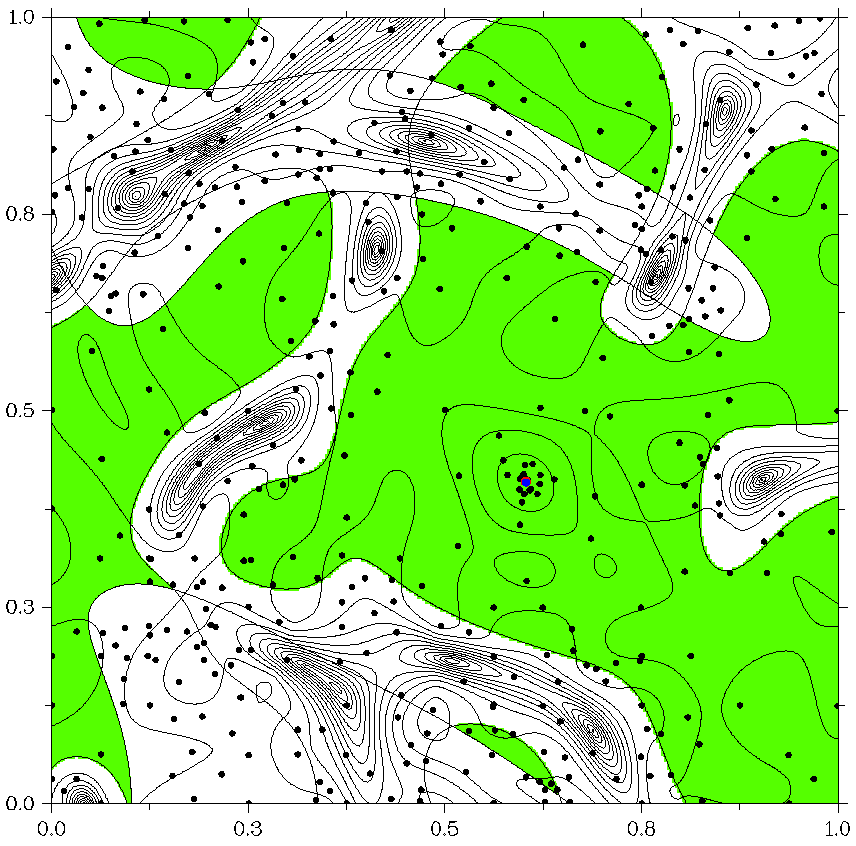
\includegraphics[width=.5\textwidth]{pic/2.png}}}
    \subfloat[Solution at the boundary of feasible area]{
    {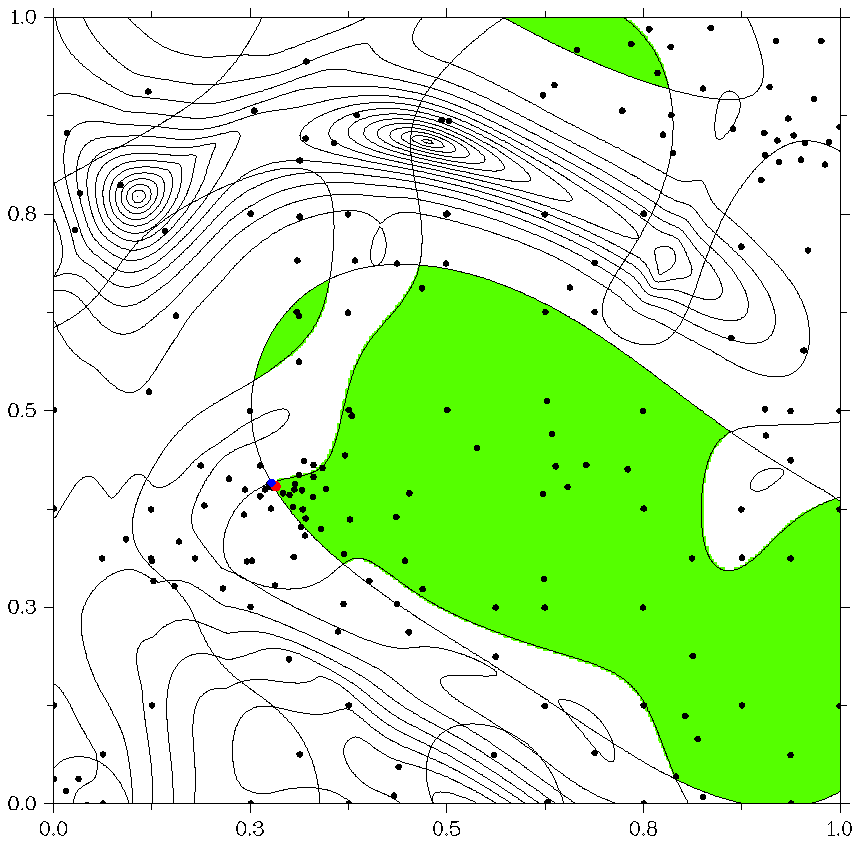
\includegraphics[width=.5\textwidth]{pic/4.png}}}
    \caption{Contour plots and trial points of IAGS in two synthetic problems}
    \label{fig:isolines}
\end{figure}

A test problem was considered to be solved if the optimization method executes the next trial
\(y^k\) in the \(\delta\)-vicinity of the global minimizer \(y^*\), i.e.
\(\left\|y^k-y^*\right\|\leqslant \delta = 0.01\left\|b-a\right\|\),
where \(a\) and \(b\) are the left and right boundaries of the hypercube from (\ref{eq:task}).
If this relation is not fulfilled upon reaching the limit of number of iterations, the problem was
considered to be not solved.

When evaluating the quality of the method and its implementation, besides the speedup due to
the parallelization and the work time,
Was taken into account as well.
The mean maximum distance (in terms of \(l_{\infty}\)-norm) form the current estimate of the
optimum to its actual position computed on the set of problems (\ref{eq:many_problems}):
\(D_{avg}\) and \(D_{max}\).
The dynamics of these magnitudes in the course of the optimization shows how uniformly the
method distributes the resources among the problems.

The parallel method was implemented on C++ language with the use OpenMP technology for
the parallelization of the trial execution process in the shared memory.
All numerical experiments were carried out using a computer with the following  configuration:
Intel Core i7-7800X, 64GB RAM, Ubuntu 16.04 OS, GCC 5.5 compiler.

\subsection{Result of solving the generated problems}

The results of solving the test problems by the sequential and parallel versions of the modified
IAGS for solving the sets of problems are presented in Table~\ref{tab:speedup}.
For all two-dimensional classes of problems, the parameter \(r=4.7\).
In the case of the three-dimensional problems, \(r=4.7\) and also to improve the convergence speed
\(\varepsilon\)-reservation technique from \cite{Strongin2000} Chapter 8.3 with
\(\varepsilon=0.1\) has been employed.
In all experiments, an additional computational load was introduced into the objective function
and constraints so that the time of a single call of a problem function was equal to
approximately 1 ms.

One can see from Table \ref{tab:speedup} that the speedup in the iterations \(S_i\) increased
linearly with increasing number of threads \(p\) whereas the speedup in time \(S_t\) increased
not so fast that points to a non-ideal implementation of the algorithm.
One can increase the actual speedup, the upper limit for which is \(S_i\) by the optimization of
the interaction between the copies of IAGS. It is planned to do in the course of future work.

\begin{table}
  \centering
  \caption{Results of experiments on the sets of synthetic problems}
  \label{tab:speedup}
  \begin{tabular}{c|c|cccc}
    %\cline{1-8}\noalign{\smallskip}
    Problem class & \textit{p} & Number of iterations & Time, s & \(S_i\) & \(S_t\)   \\
    %s\noalign{\smallskip} \cline{4-5} \cline{7-8}  \noalign{\smallskip}
    \hline
    GKLS \& \(F_{GR}\) based \
      & 1 & 51434 & 90.20 & -    & - \\
      & 2 & 25698 & 56.96 & 2.00 & 1.58 \\
      & 4 & 13015 & 36.67 & 3.95 & 2.46 \\
      & 6 & 8332  & 26.85 & 6.17 & 3.36 \\
    \hline
    GKLS based 2d \
      & 1 & 59066 & 97.53 & -    & - \\
      & 2 & 29060 & 60.56 & 2.04 & 1.61 \\
      & 4 & 14266 & 38.92 & 4.14 & 2.51 \\
      & 6 & 9436  & 29.53 & 6.26 & 3.30 \\
    \hline
    GKLS based 3d \
      & 1 & 782544 & 1117.55 & -    & - \\
      & 2 & 397565 & 752.92  & 1.97 & 1.48 \\
      & 4 & 208073 & 526.67  & 3.76 & 2.12 \\
      & 6 & 142089 & 445.45  & 5.50 & 2.51 \\
    \hline
  \end{tabular}
\end{table}

In order to demonstrate the uniform convergence, all test problems have been solved by IAGS
in the regime of solving separate problems as well.
Fig. \ref{fig:devs_mixed} presents the plots of mean and maximum distances from the actual
optima to the current estimates of these ones when solving a series of problems generated by
two different generators separately (solid line) and together (dashed line).
In spite of an essential differences in the structure of problems, the modified IAGS decreased
the maximum deviations of the estimates from the optima as well as the mean ones much faster.
It evidences the uniform convergence over the whole set of problems being solved all together.
At that, in the case of the sequential solving of the problems, the magnitude \(D_{max}\) takes
its maximum value until the last problem is solved.

\begin{figure}[ht]
    \centering
    \subfloat[\(D_{max}\)]{
    \label{fig:max_dev} {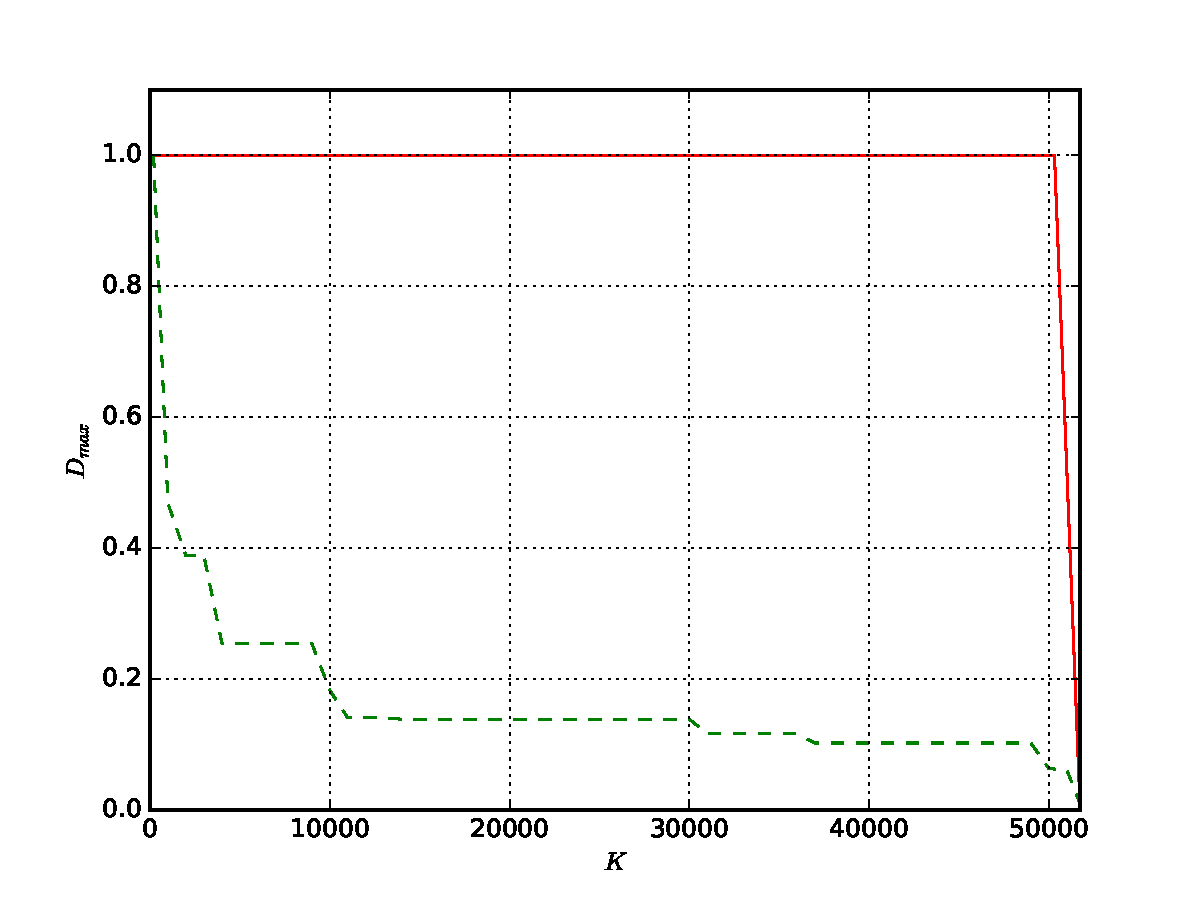
\includegraphics[width=.5\textwidth]{pic/mixed_2d_max.pdf}}}
    \subfloat[\(D_{avg}\)]{
    \label{fig:avg_dev} {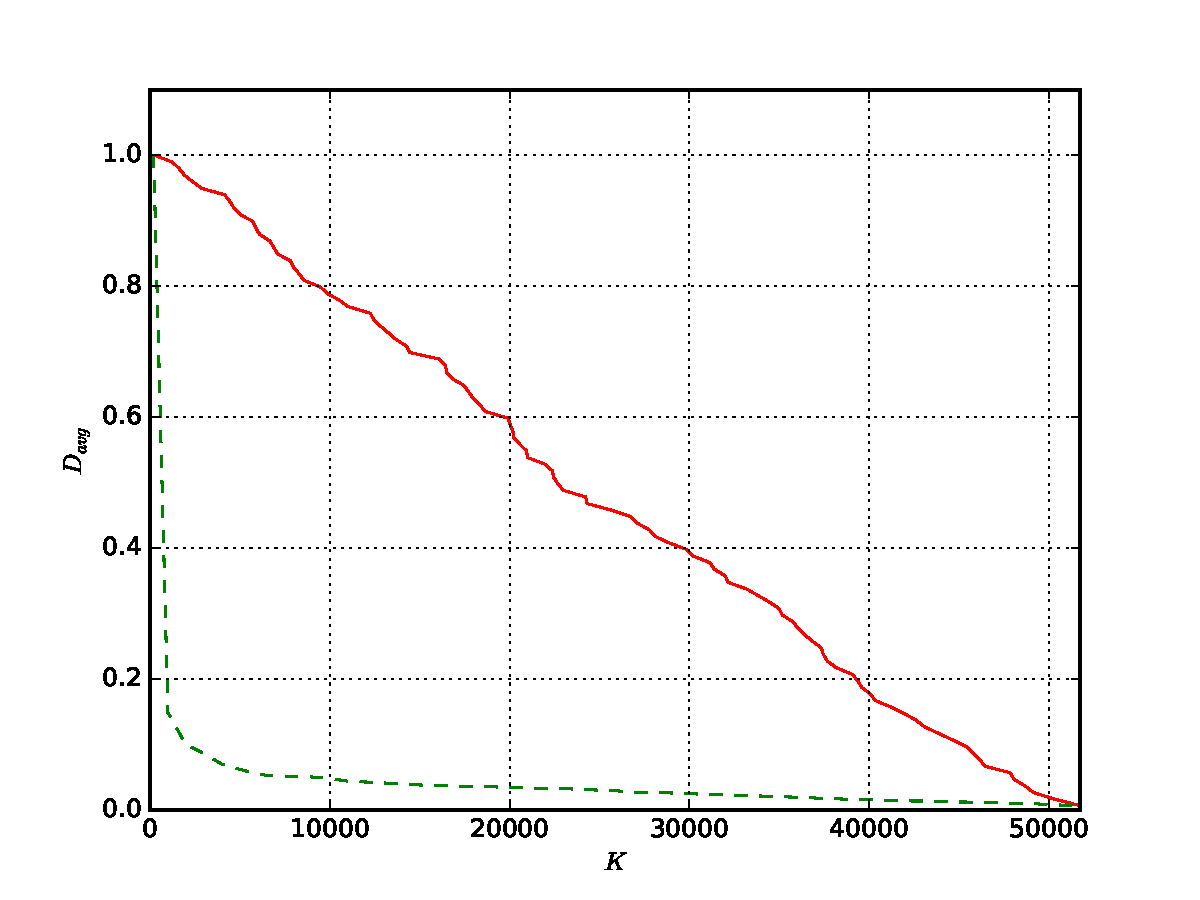
\includegraphics[width=.5\textwidth]{pic/mixed_2d_avg.pdf}}}
    \caption{Dynamics of \(D_{avg}\) and \(D_{max}\) in the course of solving a set of the two-
dimensional problems generated by two different generators GKLS and \(F_{GR}\)}
    \label{fig:devs_mixed}
\end{figure}

\subsection{Example of solving a multicriteria problems}

In order to demonstrate the efficiency of the approach to the balancing of the load, let us
consider an example, in which a set of problems of the kind (\ref{eq:many_problems}) is
generated as a result of scalarization of a multicriteria optimization problem with constrains.

Let us consider a test problem from \cite{BinhKorn1999}:
\begin{equation}
  \label{eq:mco_probem}
  \begin{array}{l}
      Minimize \left \{
      \begin{array}{l}
        f_1(y) = 4 y_1^2 + 4 y_2^2 \\
        f_2(y) = (y_1-5)^2 + (y_2-5)^2 \\
      \end{array}
      \right .
      , y_1\in [-1,2],y_2\in [-2,1],
      \\s.t.
      \\
      \left \{
      \begin{array}{l}
        g_1(y) = (y_1 - 5)^2 + y_2^2 - 25 \leqslant 0, \\
        g_2(y) = -(y_1 - 8)^2 - (y_2 + 3)^2 + 7.7 \leqslant 0.\\
      \end{array}
      \right .
  \end{array}
\end{equation}

Let us use the Germeyer convolution for the scalarization of the problem
(\ref{eq:mco_probem}).
After the convolution, the scalar objective function takes the form:
\begin{equation}
  \varphi(y,\lambda_1,\lambda_2)=\max\{\lambda_1 f_1(y), \lambda_2 f_2(y)\},
\end{equation}
where \(\lambda_1,\lambda_2\in[0,1],\: \lambda_1+\lambda_2=1\).
Trying all possible convolution coefficients, one can find the whole set of Pareto-optimal
solutions in the problem (\ref{eq:mco_probem}).
For the numerical construction of the Pareto set, let us select 100 sets of coefficients
\((\lambda_1,\lambda_2)\) so that
\(\lambda_1^i=i h,\: \lambda_2^i=1-\lambda_1^i,\: h=10^{-2},\: i=\overline{1, 100}\).

As the limitation for the computational resources, a limit of 2500 trials was selected.
The set of auxiliary scalar problems was solved by two methods:
\begin{itemize}
  \item each problem was solved separately using IAGS with a preset limit of 25 trials. This way,
the computational resources were distributed among the problems uniformly;
  \item all problems are solved simultaneously using generalized IAGS with a preset limit of
2500 trials.
\end{itemize}
In both cases, the parameter \(r=4\).

\begin{figure}[ht]
    \centering
    \subfloat[IAGS, separate solving of the problems]{
    \label{fig:mco_pareto_1} {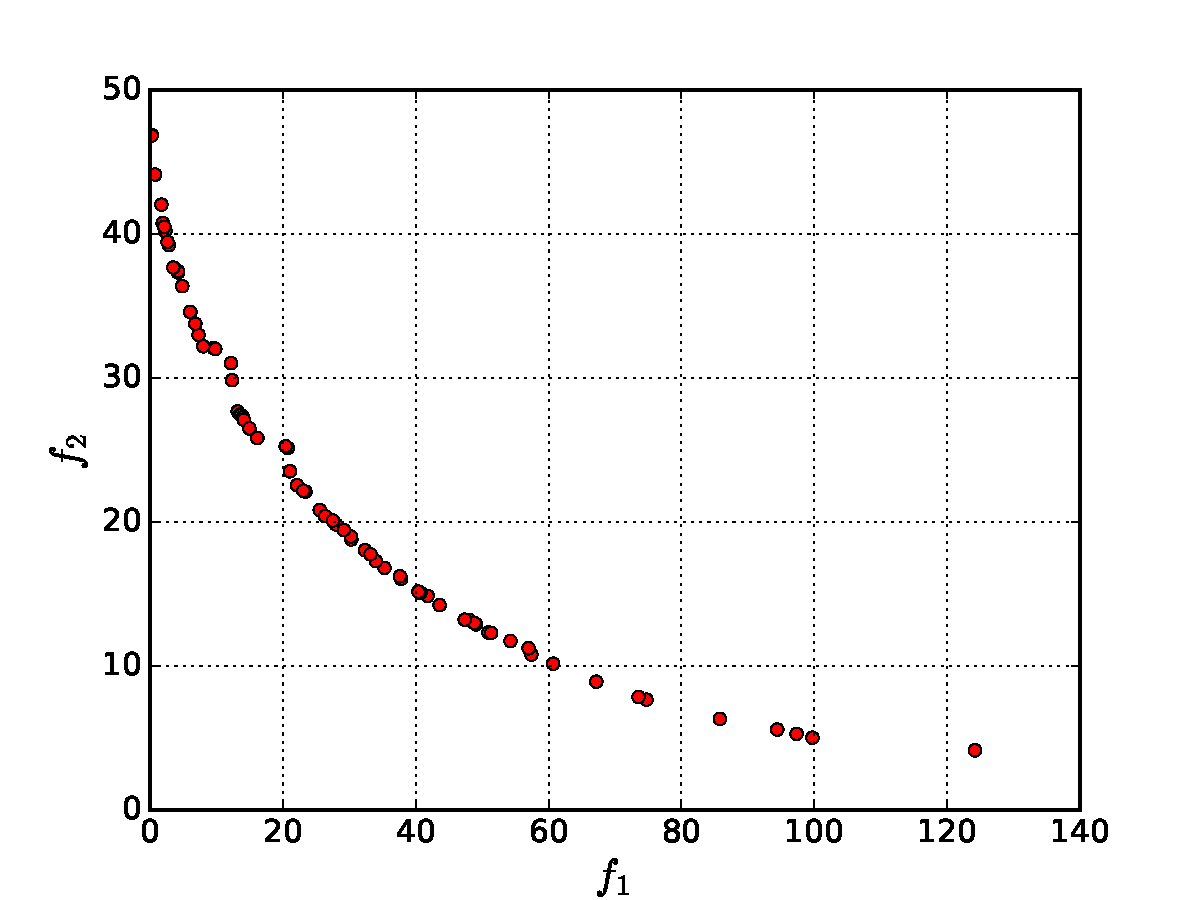
\includegraphics[width=.5\textwidth]{pic/single_mco.pdf}}}
    \subfloat[IAGS for the set of problems]{
    \label{fig:mco_pareto_2} {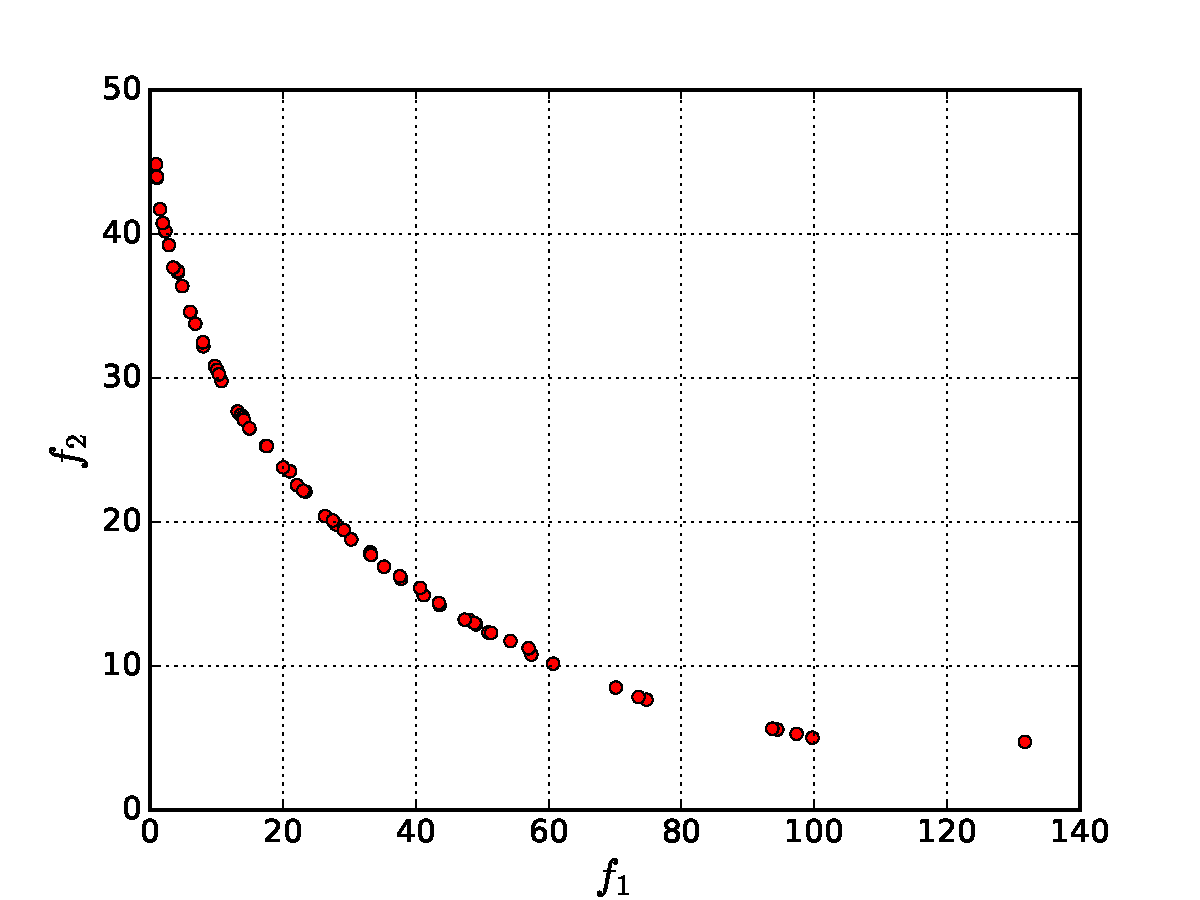
\includegraphics[width=.5\textwidth]{pic/multi_mco.pdf}}}
    \caption{Numerical estimates of Pareto set in the problem (\ref{eq:mco_probem}), obtained
after 2500 trials}
    \label{fig:mco_pareto}
\end{figure}

The plots of solutions obtained by each method are presented in Fig. \ref{fig:mco_pareto_1}
and Fig. \ref{fig:mco_pareto_2}.
All plots agree with the ones presented in \cite{BinhKorn1999} qualitatively (the authors
haven't provided any other information to compare).
One can see the Pareto curve in Fig. \ref{fig:mco_pareto_1} to have concavities that doesn't
match the solution presented in \cite{BinhKorn1999} and means the lack of resources for
solving some auxiliary problems.
To evaluate the quality of solution, the index \(Spacing(SP)\) \cite{RiquelmeLucken2015}
featuring the density of the points approximating the Pareto set was computed also.
\begin{equation*}
\begin {array}{l}
  SP(S)=\sqrt{\frac{1}{|S|-1} \sum_{i=1}^{|S|} (\overline{d}-d_i)^2},
  \; \overline{d}=mean\{d_i\},
  \\d_i=\min_{s_i,s_j\in S:s_i\ne s_j}||F(s_i)-F(s_j)||_1,\; F=(f_1,f_2).
  \end{array}
\end{equation*}
In the case of separate solving of the problem \(SP_{single}=0.984\) whereas when solving of
the problems by the method with the balancing of the load \(SP_{multi}=0.749\) that evidences
a better quality of the approximation of the solution.

\section{Conclusion}

In the course of present work, the support of the non-convex constraints was implemented in the
algorithm solving a set of the global optimization problems.
Also, the sufficient conditions of convergence for the developed method were obtained.
The numerical experiments demonstrating the advantages of the considered approach over
solving the problems separately were carried out.
The efficiency of solving a set of problems together was demonstrated by the example of
solving a multicriteria problem with nonlinear constraints.

In the course of further work, it is planned to improve current implementation of the algorithm
by reducing the costs of supporting the search information for the set of problems and, this way,
improving the indices of time speedup due to the parallelization.
Also, it is planned to implement a version of considered algorithm working in the distributed
memory according to the scheme described in \cite{BarkalovLebedev2017_2}.

%
% ---- Bibliography ----
%
% BibTeX users should specify bibliography style 'splncs04'.
% References will then be sorted and formatted in the correct style.
%
\bibliographystyle{splncs04}
\bibliography{bibliography}
%
\end{document}
